% !TeX spellcheck = fr_FR
\chapter{Chapitre 1 : Analyse}

\section{Description du projet}
Votre texte, votre texte, votre texte, votre texte, votre texte, votre texte, votre texte, votre texte, votre texte, votre texte, votre texte, votre texte, votre texte, votre texte, votre texte, votre texte, votre texte, votre texte.

\section{Méthodes de communication}
Votre texte, votre texte, votre texte, votre texte, votre texte, votre texte, votre texte, votre texte, votre texte, votre texte, votre texte, votre texte, votre texte, votre texte, votre texte, votre texte, votre texte, votre texte.
\subsection{UART}
\subsection{PCIe}
\subsection{Ethernet}

\section{Bcrypt}

Pour ce projet, nous avons décidé de cibler le Bcrypt, car c'est une fonction de hachage qui prend du temps à être calculé. 

Le Bcrypt est une fonction de hachage avec comme particularité, un paramètre supplémentaire qui est le cost (coût en français).
Ce paramètre va définir le nombre d'itérations que va prendre la fonction de hachage, de ce fait plus le cost est élevé, plus le calcul va prendre du temps.

\subsection{Algorithme}

L'algorithme du Bcrypt se base sur l'algorithme de chiffrement Blowfish\footcite{noauthor_blowfish_2019} qui est une fonction de chiffrement à clef symétrique, c'est-à-dire que la même clef est utilisée pour le chiffrement et le déchiffrement. 
L'algorithme du Bcrypt peut être divisé en deux grandes étapes.

On a une première étape qui est une phase de mise en place des clés symétriques. 
Dans cette étape, on va créer les clés de chiffrements à partir des paramètres d'entrée de la fonction de hachage (mot de passe, salt, cost). 
Cette première étape est la partie la plus coûteuse de la fonction, car la mise en place de la clé va prendre plus ou moins de temps en fonction du cost. 
Les clés de chiffrement sont composées de Subkeys qui est un tableau de 18 entiers de 32 bits et quatre \gls{sbox} qui sont chacun des tableaux de 256 entiers de 32 bits. 
Avant de calculer ces clés de chiffrements, ils sont tout d'abord initialisés avec les décimales de PI.

Puis il y a la deuxième étape, où l'on va utiliser les clés de chiffrement qui ont été calculées plus tôt afin de chiffrer la phrase magique "OrpheanBeholderScryDoubt", le chiffrement va être fait 64 fois.

\begin{figure}[tbph!]
	\centering
	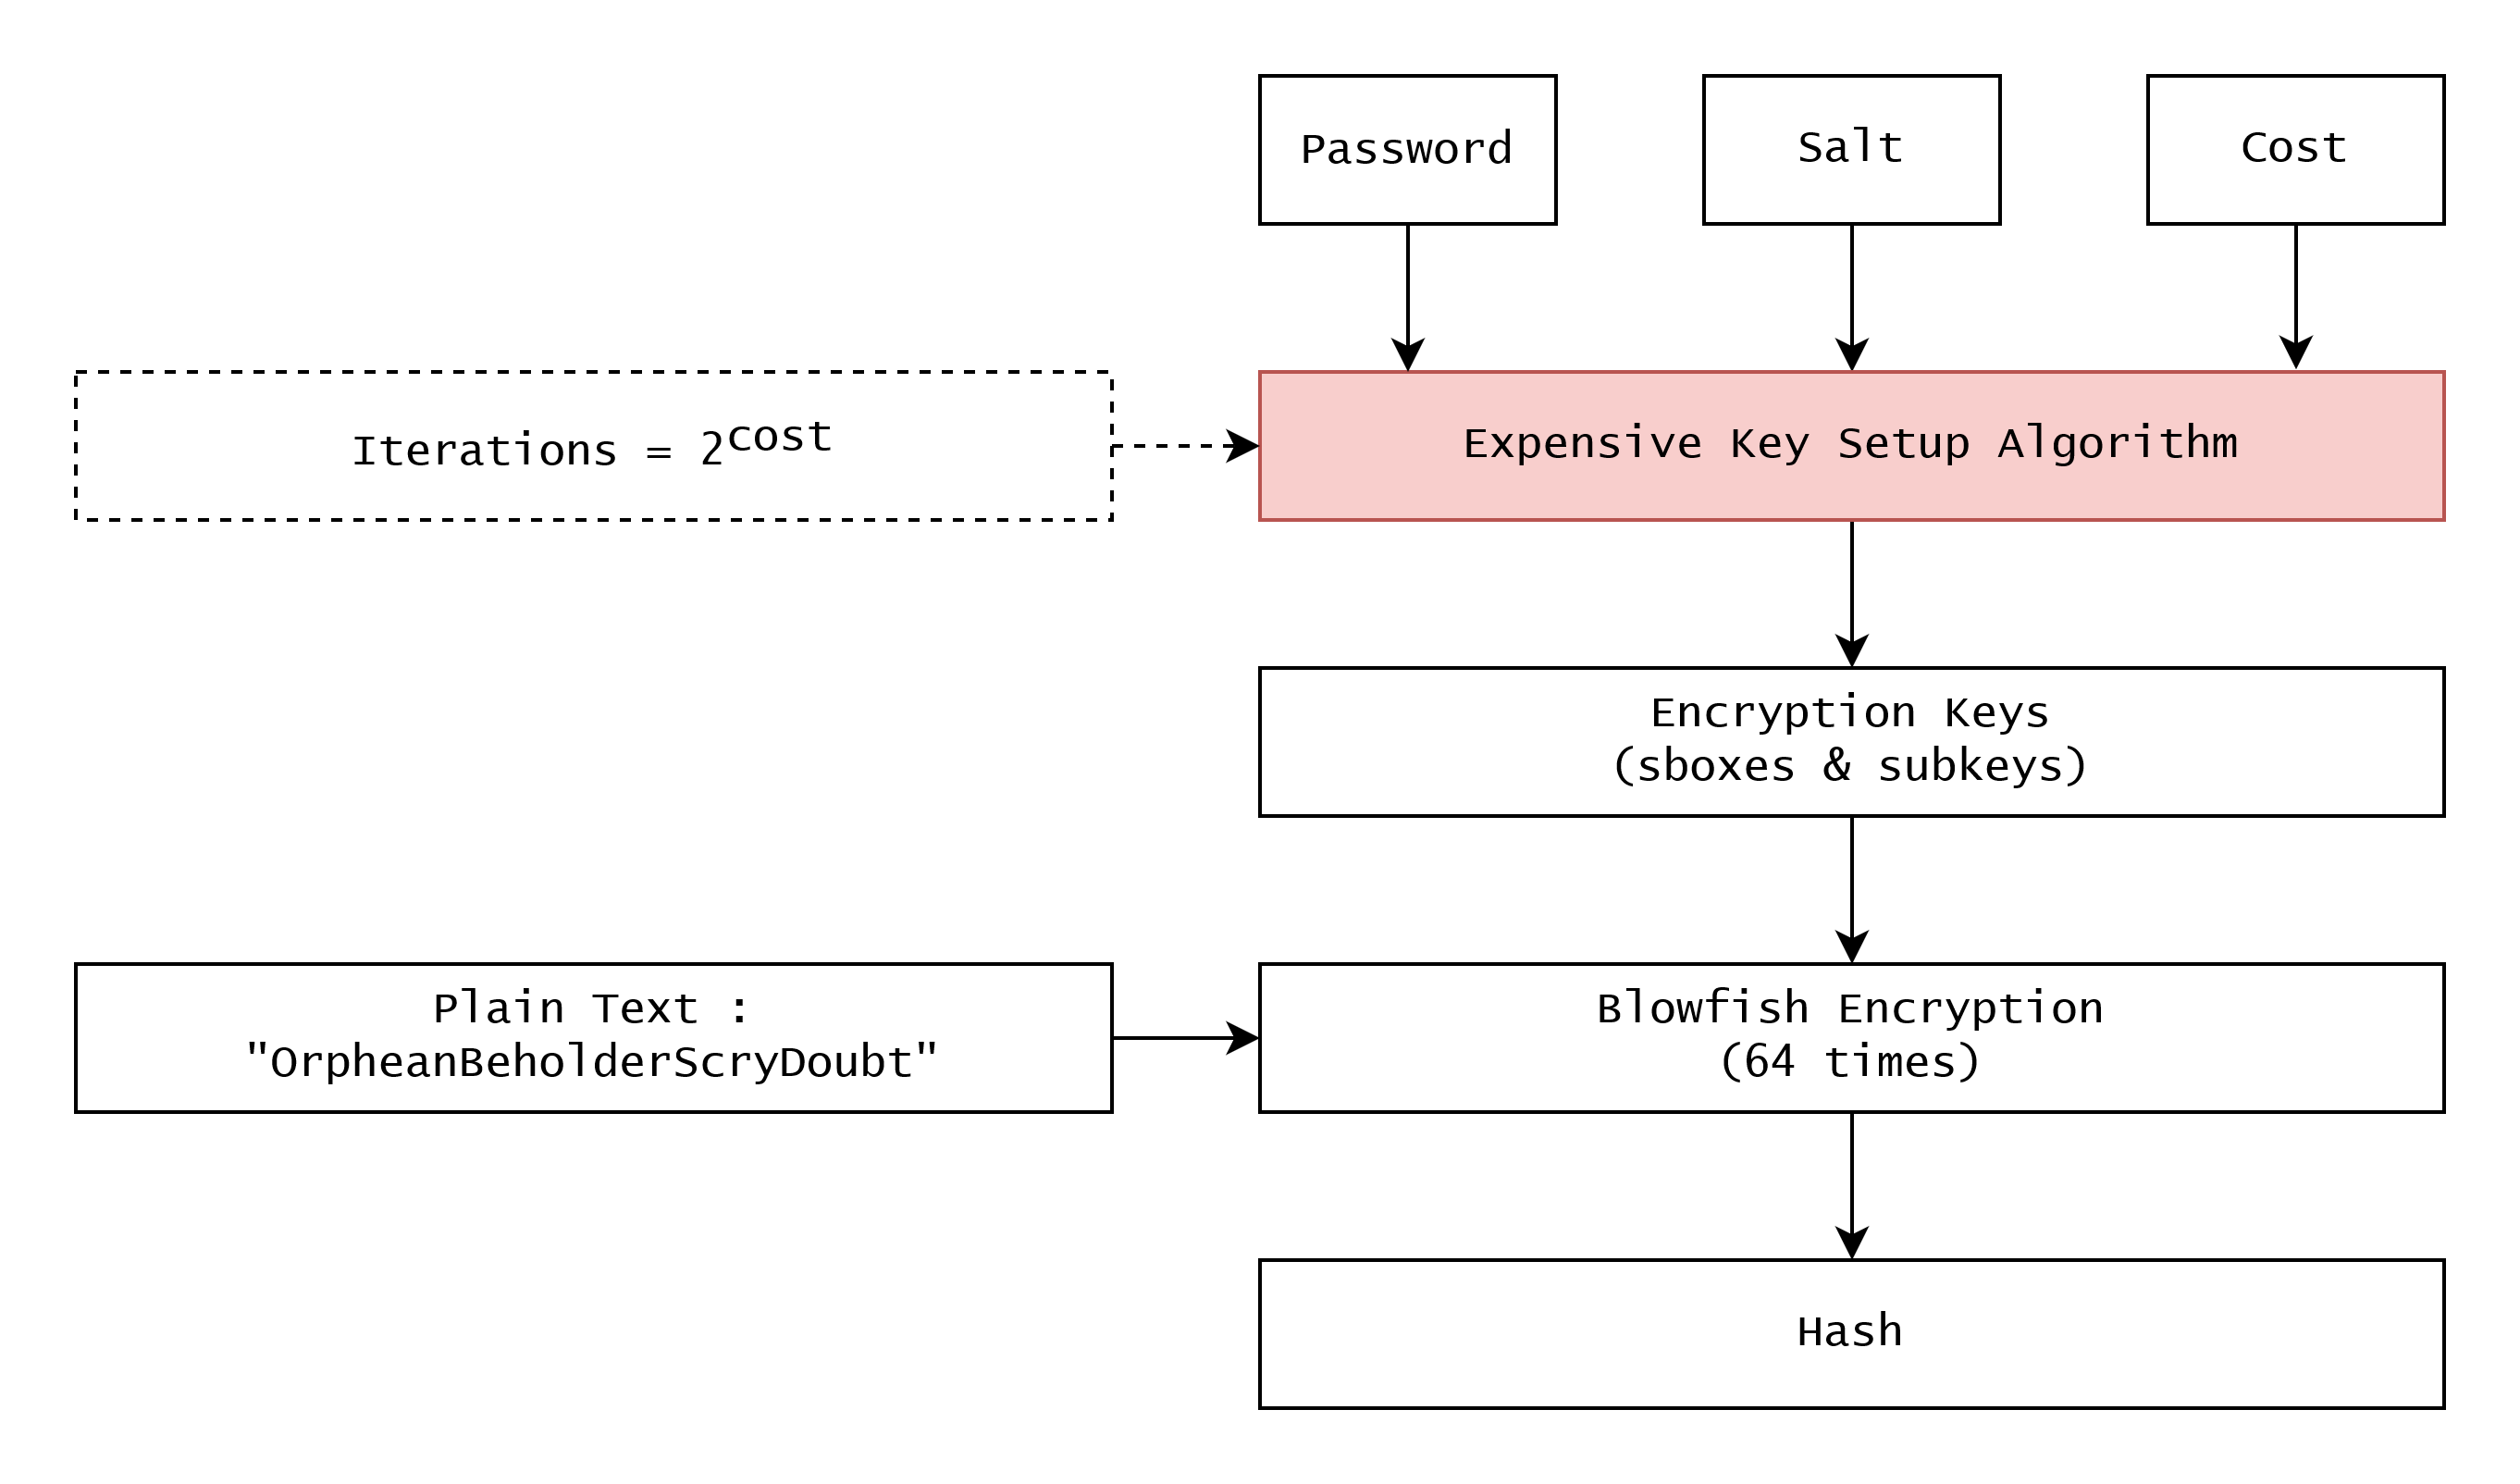
\includegraphics[width=0.7\linewidth]{bcrypt_algo}
	\caption[Algorithme Bcrypt]{Algorithme Bcrypt. Source : réalisé par Kandiah Abivarman}
	\label{fig:bcrypt_algo}
\end{figure}

\newpage

\subsection{Format du Hash}

Le hash généré par la fonction Bcrypt est généralement stocker sous une forme particulière. 

\begin{figure}[tbph!]
	\centering
	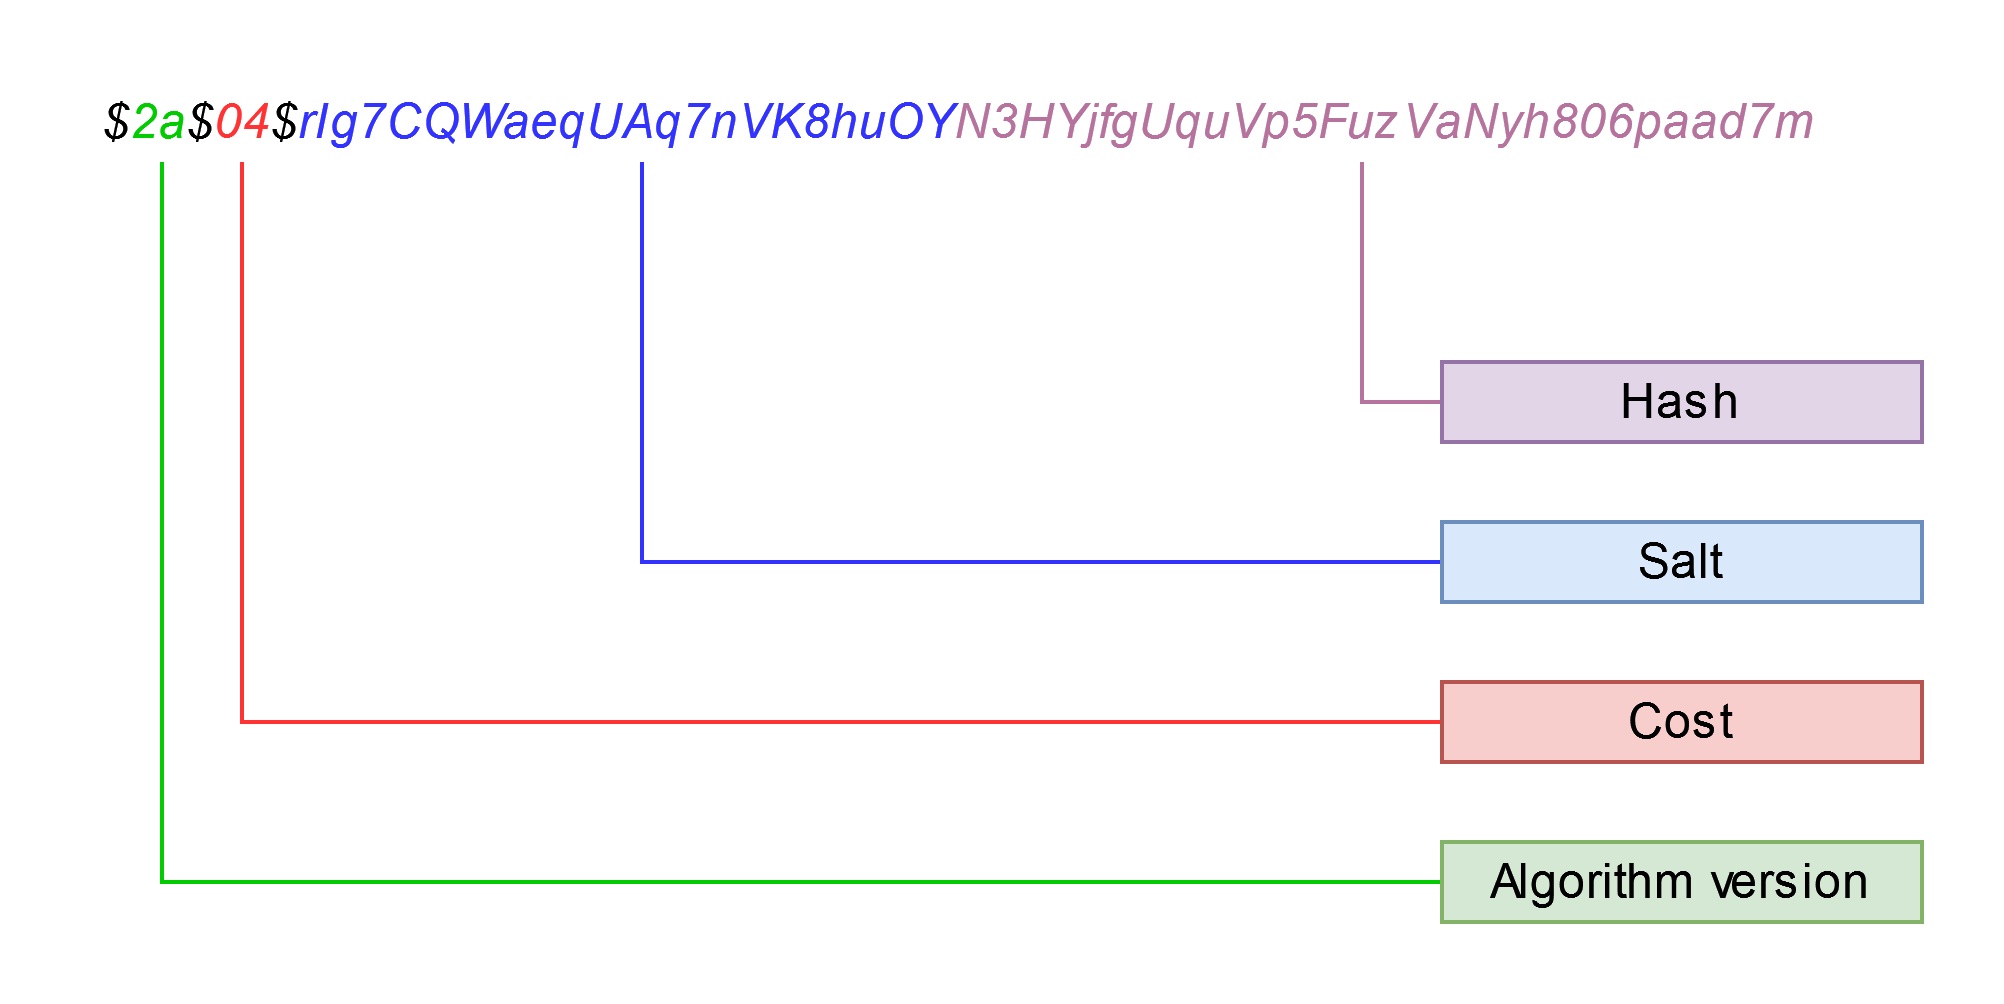
\includegraphics[width=0.7\linewidth]{bcrypt_hash_format}
	\caption[Format du hash Bcrypt]{Format du hash Bcrypt. Source : réalisé par Kandiah Abivarman}
	\label{fig:bcrypt_hash_format}
\end{figure}

On va avoir un premier champ qui contient la version de l'algorithme, un deuxième qui contient le cost de la fonction, un troisième avec le salt et le quatrième avec le hash généré. 
Le salt et le hash sont en base 64, mais il faut faire attention, car c'est une base 64 différente de la norme RFC 4648\footcite{josefsson_base16_2006} qui est couramment utilisé.

\begin{figure}[tbph!]
	\centering
	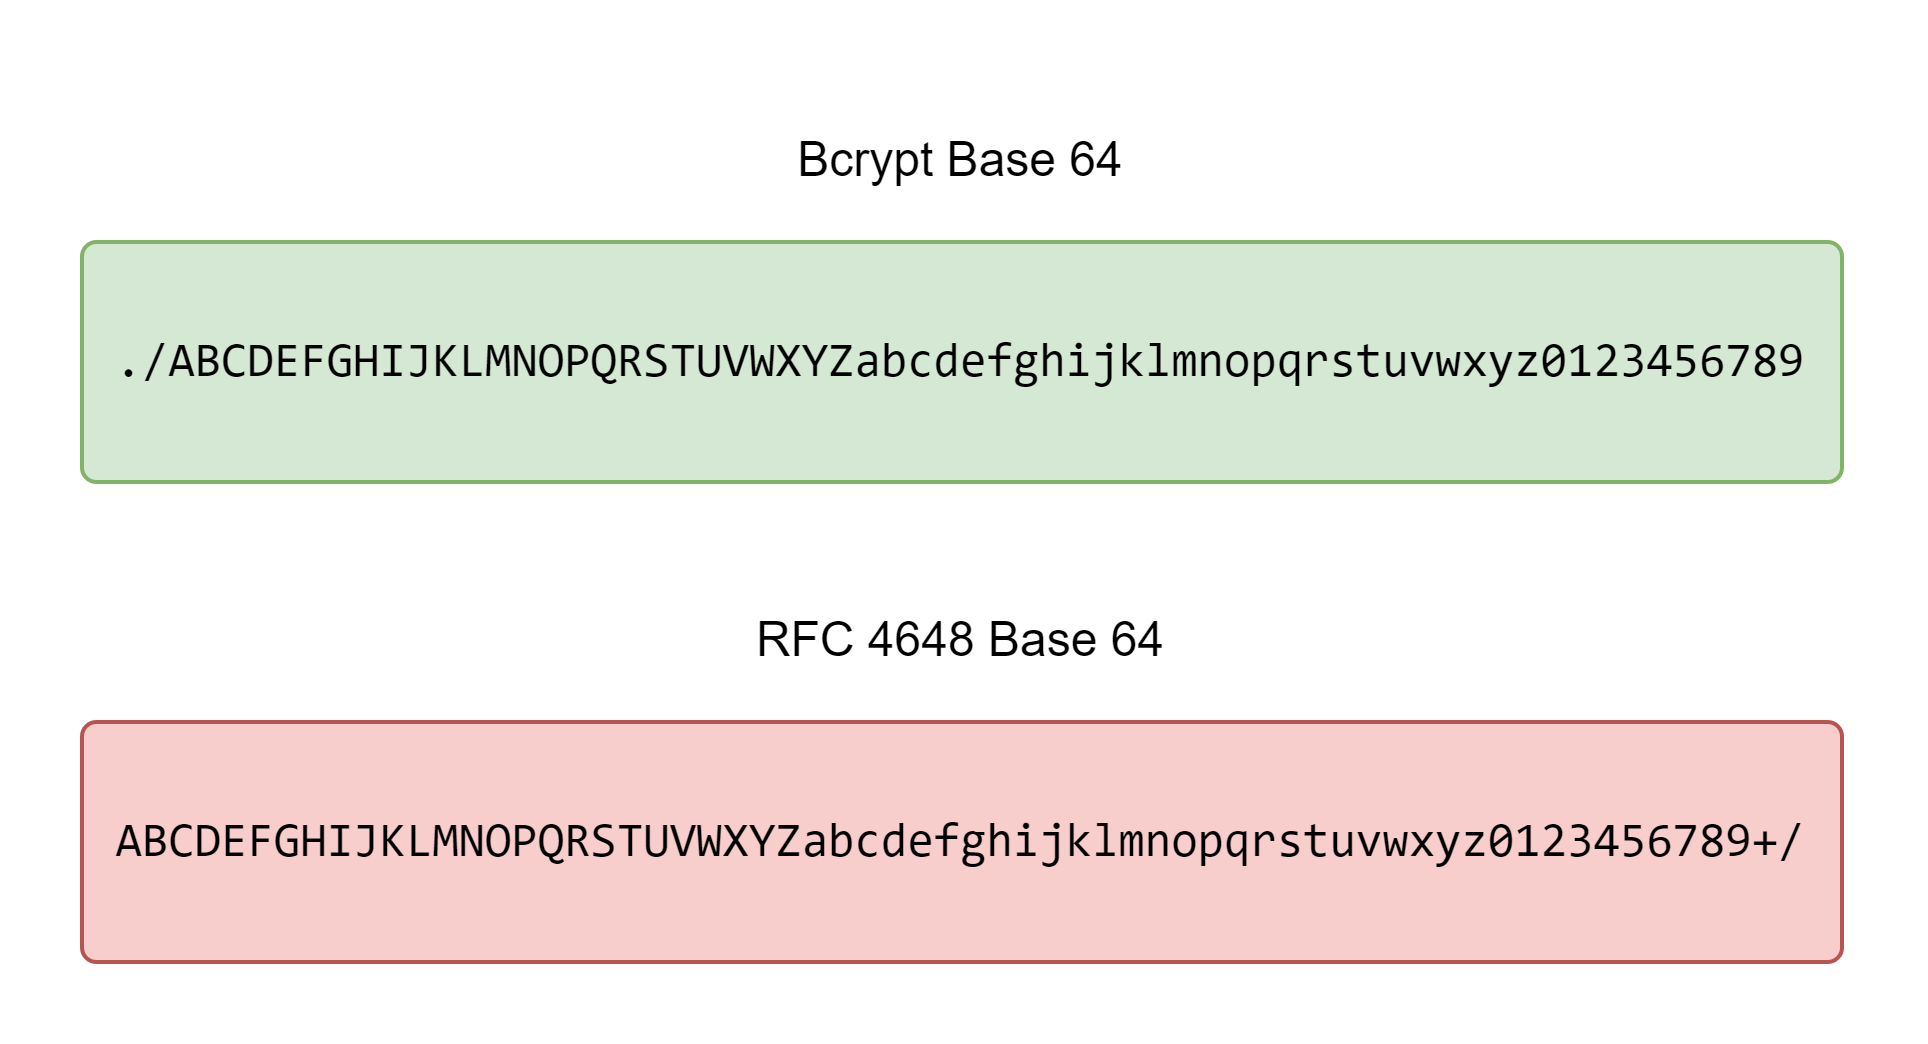
\includegraphics[width=0.7\linewidth]{base_64}
	\caption[Différence Base 64]{Différence Base 64. Source : réalisé par Kandiah Abivarman}
	\label{fig:base_64}
\end{figure}

\section{Projet de semestre}
Votre texte, votre texte, votre texte, votre texte, votre texte, votre texte, votre texte, votre texte, votre texte, votre texte, votre texte, votre texte, votre texte, votre texte, votre texte, votre texte, votre texte, votre texte.
